\chapter{Diagramas en \LaTeX{}}
Sorprendentemente hay varios tipos de diagramas en \LaTeX{},
el principal paquete para lograr ésto es Ti$k$Z y sus aplicaciones varian dependiendo del tipo de diagrama y de su complejidad.
Primero veremos aplicaciones sencillas como diagramas conmutativos, algunos tipos de gráficos y luego veremos cosas más especificas.
Éste capítulo principalmente constara de ejemplos sin mucha explicación.

Así que añadimos a la cabecera:
\begin{lstlisting}
\usepackage{tikz}
\usetikzlibrary{babel}
\end{lstlisting}
La segunda línea introduce la librería \texttt{babel} de Ti$k$Z que evita problemas con el paquete \texttt{babel}.

\section{Diagramas conmutativos}
Para hacer diagramas conmutativos usaremos la librería \texttt{cd} así que en una sóla línea es:
\begin{lstlisting}
\usetikzlibrary{cd}
\end{lstlisting}
Éste provee el entorno \texttt{tikzcd} que admite argumentos opcionales.
En él, los símbolos se muestran automáticamente en modo matemático y se ordenan en forma de tabla con celdas (separados por \texttt{\&}).
Para dibujar flechas se usa el comando \lstinline|\arrow| o \lstinline|\ar| para acortar.
Toda la información va en un campo opcionar, comenzando por la dirección de la flecha
(\texttt{l} izquierda, \texttt{r} derecha, \texttt{u} arriba, \texttt{d} abajo),
luego una coma y entre comillas el contenido de la flecha.

Entre las comas, puedes poner el color de la flecha si así se quiere.
Si las comillas terminan en un apostrofe entonces el contenido saldrá al otro lado de lo esperado y si se utiliza la opción \texttt{description}
entonces aparece en el medio.
\begin{lstlisting}
\begin{tikzcd}
	A \ar[r, "f"] \ar[rd, "f\circ g"'] & B \ar[d, "g"]\\
	                                   & C
\end{tikzcd}
\end{lstlisting}
\begin{center}
	\begin{tikzcd}
		A \ar[r, "f"] \ar[rd, "f\circ g"'] & B \ar[d, "g"]\\
		                                   & C
	\end{tikzcd}
\end{center}
Además se pueden abreviar los movimientos anteponiendo el movimiento en el nombre del comando, e.g., \lstinline|\rar| reemplaza a \lstinline|\ar[r]|.
En caso de los movimientos diagonales, la componente vertical va primero, e.g., \lstinline|\rdar| no se admite, pero \lstinline|\drar| sí.
No obstantem movimientos más complicados deben ser declarados: no existe \lstinline|\rrar|, ni \lstinline|\ddlar| por ejemplo.

Para cambiar la separación de columnas y filas están las opciones de \texttt{column sep} y \texttt{row sep} respectivamente
que pueden igualar a uno de los siguientes tamaños (de menor a mayor):
\begin{center}
	\ttfamily tiny, small, scriptsize, normal, large, huge.
\end{center}
Y los tipos de flechas son:
\begin{center}
	\begin{tabular}{ll|ll}
		\hline \hline
		\texttt{to head}    & \begin{tikzcd}\rar[to head]&{}\end{tikzcd} & \texttt{Rightarrow} & \begin{tikzcd}\rar[Rightarrow]&{}\end{tikzcd} \\
		\texttt{maps to}    & \begin{tikzcd}\rar[maps to]&{}\end{tikzcd} & \texttt{Mapsto}     & \begin{tikzcd}\rar[Mapsto]&{}\end{tikzcd} \\
		\texttt{hook}       & \begin{tikzcd}\rar[hook]&{}\end{tikzcd}    & \texttt{hook'}      & \begin{tikzcd}\rar[hook']&{}\end{tikzcd} \\
		\texttt{tail}       & \begin{tikzcd}\rar[tail]&{}\end{tikzcd}    & \texttt{two heads}  & \begin{tikzcd}\rar[two heads]&{}\end{tikzcd} \\
		\texttt{dashed}     & \begin{tikzcd}\rar[dashed]&{}\end{tikzcd}  & \texttt{squiggly}   & \begin{tikzcd}\rar[squiggly]&{}\end{tikzcd} \\
		\texttt{harpoon}    & \begin{tikzcd}\rar[harpoon]&{}\end{tikzcd} & \texttt{harpoon'}   & \begin{tikzcd}\rar[harpoon']&{}\end{tikzcd} \\
		\hline \hline
	\end{tabular}
\end{center}
Un programa muy útil para hacer diagramas conmutativos y que genera el código para copiar y pegar es \url{https://tikzcd.yichuanshen.de/}.

\pagebreak
\subsection{Primer teorema de isomorfismos}
\begin{lstlisting}
\begin{tikzcd}[row sep=large, column sep=tiny]
	G \ar[rr, "\varphi", two heads] \drar["\pi"', two heads] &  & H \\
	& G/\ker\varphi \urar["\exists!\bar\varphi"', dashed]
\end{tikzcd}
\end{lstlisting}
\begin{center}
	\begin{tikzcd}[row sep=large, column sep=tiny]
		G \ar[rr, "\varphi", two heads] \drar["\pi"', two heads] &  & H \\
		& G/\ker\varphi \urar["\exists!\bar\varphi"', squiggly]
	\end{tikzcd}
\end{center}

\subsection{Kernels (según teoría de categorías)}
\begin{lstlisting}
\begin{tikzcd}[row sep=large]
	& X \drar["f"] \\
	& K \uar["k"'] \rar["0_{KY}"] & Y \\
	K' \urar["u" description, dotted] \ar[uur, "k'", shift left] \ar[urr, "0_{K'Y}"', shift right]
\end{tikzcd}
\end{lstlisting}
\begin{center}
	\begin{tikzcd}[row sep=large]
		& X \drar["f"] \\
		& K \uar["k"'] \rar["0_{KY}"] & Y \\
		K' \urar["u" description, dotted] \ar[uur, "k'", shift left] \ar[urr, "0_{K'Y}"', shift right]
	\end{tikzcd}
\end{center}

[Fuente: \Href{https://en.wikipedia.org/wiki/Kernel_(category_theory)}{Wikipedia}]

\subsection{Lema de la serpiente}
Éste ejemplo emplea la librería de Ti$k$Z \texttt{calc} para calcular la posición de la flecha roja,
lo único diferente es de hecho la misma flecha que ocupa el método \texttt{controls} que funciona como los controladores de curvas de Bézier.
También el código asume que se ha definido el operador \lstinline|\coker| que hace lo que se espera.
\begin{lstlisting}
\begin{tikzcd}[row sep=large]
	0 \rar[red] & \ker f \rar[red] & \ker\alpha \dar \rar[red] & \ker\beta \dar \rar[red] & \ker\gamma \dar \ar[llddd, "s"', red, controls={+(4, 0) and ($(\tikztotarget)+(-4,0)$)}] \\
	& & A \dar[blue, "\alpha"] \rar[blue, "f"] & B \rar[blue, "g"] \dar[blue, "\beta"] & C \rar[blue] \dar[blue, "\gamma"] & 0 \\
	& 0 \rar[blue] & A' \rar[blue, "f'"'] \dar & B' \rar[blue, "g'"'] \dar & C' \dar \\
	& & \coker\alpha \rar[red] & \coker\beta \rar[red] & \coker\gamma \rar[red] & \coker g' \rar[red] & 0
\end{tikzcd}
\end{lstlisting}
\begin{center}
	\begin{tikzcd}[row sep=large]
		0 \rar[red] & \ker f \rar[red] & \ker\alpha \dar \rar[red] & \ker\beta \dar \rar[red] & \ker\gamma \dar \ar[llddd, "s"', red, controls={+(4, 0) and ($(\tikztotarget)+(-4,0)$)}] \\
		& & A \dar[blue, "\alpha"] \rar[blue, "f"] & B \rar[blue, "g"] \dar[blue, "\beta"] & C \rar[blue] \dar[blue, "\gamma"] & 0 \\
		& 0 \rar[blue] & A' \rar[blue, "f'"'] \dar & B' \rar[blue, "g'"'] \dar & C' \dar \\
		& & \coker\alpha \rar[red] & \coker\beta \rar[red] & \coker\gamma \rar[red] & \coker g' \rar[red] & 0
	\end{tikzcd}
\end{center}

[Fuente: \Href{https://mathworld.wolfram.com/SnakeLemma.html}{MathWorld}]

\section{Gráficos}
Para hacer gráficos ya sea de funciones o de datos, mi principal recomendación es el paquete:
\begin{lstlisting}
\usepackage{pgfplots}
\end{lstlisting}
En general, el paquete es extremadamente amplio así que recomiendo mucho revisar el manual, si bien es largo, vale 100\% la pena por su exceso de ejemplos y
documentación, los índices explicando qué hace cada opción, y así.
En particular para evitar el exceso de opciones podemos en la cabecera definir varios estilos:
\begin{lstlisting}
\pgfplotsset{
	width = 10cm,
	compat = 1.15, % compatibilidad para compilación
	enlargelimits = false, % no extender los límites del gráfico
	grid = both, % cuadrícula
	minor tick num = 3,
	axis line style = {->}, % flechas de los ejes
	axis lines = middle, % centrar flechas en (0, 0)
	demo/.style={
		enlargelimits = true,
		grid = none,
		ticks = none
	} % demostraciones
}
\end{lstlisting}

\subsection{Funciones polinómicas y exponencial}
\begin{lstlisting}
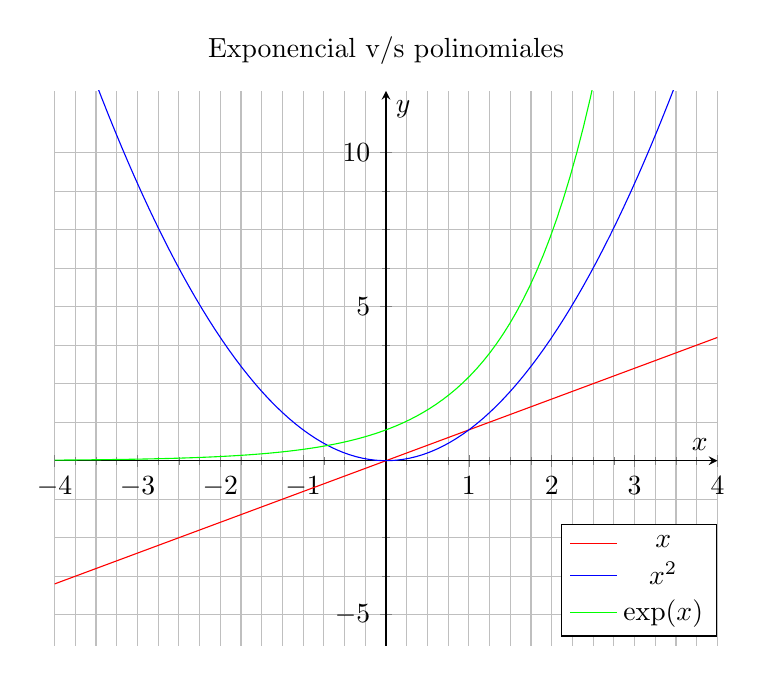
\begin{tikzpicture}
\begin{axis}[
		ymin         = -6, ymax = 12, % min/max vertical
		domain       = -4:4, % dominio
		samples      = 100,
		title        = {Exponencial v/s polinomiales},
		legend style = {at={(1, .22)}}, % ubicación de las "leyendas"
		xlabel       = {$x$}, ylabel = {$y$}]
	\addplot[red]{x};
	\addplot[blue]{x^2};
	\addplot[green]{exp(x)};
	\legend{$x$, $x^2$, $\exp(x)$} % leyendas de los gráficos
\end{axis}
\end{tikzpicture}
\end{lstlisting}
\begin{figure}[!h]
	\centering
	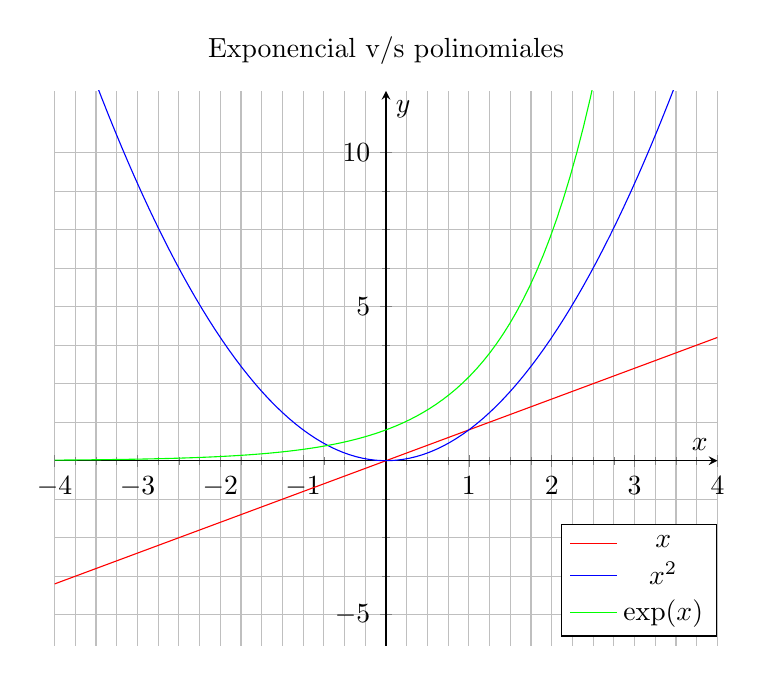
\begin{tikzpicture}
		\begin{axis}[
				ymin         = -6, ymax = 12,
				domain       = -4:4,
				samples      = 100,
				title        = {Exponencial v/s polinomiales},
				legend style = {at={(1, .22)}},
				xlabel       = {$x$}, ylabel = {$y$}]
			\addplot[red]{x};
			\addplot[blue]{x^2};
			\addplot[green]{exp(x)};
			\legend{$x$, $x^2$, $\exp(x)$}
		\end{axis}
	\end{tikzpicture}
\end{figure}
